\chapter{Discriminating sodium storage mechanisms}

This project is about using the information from the time-varying impedance to infer the mechanisms of Na storage in porous silicon carbonitride as candidate material for the negative electrode of non-aqueous Na-ion batteries. The material was developed and patented at the inorganic chemistry department of the Technical University of Darmstadt as an alternative to the most known hard carbon. This class of partially distorted and highly porous materials are expetially indicated for the storage of Na cation, as it is bigger than Li. Graphite, in fact has not enough interlayer space to accomodate Na cation. Many mechanisms for the Na cation storage into disordered structure has been proposed and it is likely that they happen all in parallel. The goal of this project was to connect the shape of the impedance with specific mechanisms and take advantage of the operando condition to get information on the potential windows this mechanisms take place. 

The material used for the project was synthesized and the electrode produce at the University of Darmstadt by Marco Melzi d’Eril.

\subsection{Silicon carbonitride}

Silicon carbonitride belongs to the catagory of polymer derived ceramic material which are obtained from the pyrolisis of preceramic polymers which are characterizxed by the heterogenous covalent bond of silicon, borono, carbon, nitrogen and oxigen giving to the final material excelnt chemical, termal and mechanical properties among them hardnes. The pirolysis procedure gives a high controll on the structure and morfology of the final product allowing to increase the porosity. The strucutre of silicon carbonitride is reported in the figure. The preceramic polymers precursor can be even manifacured as complex three-dimensinal strucuture by assitive techniques and pyrolized in a second step.
\marginpar{
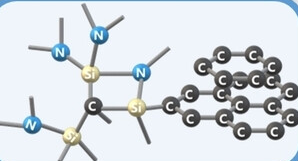
\includegraphics[width=\marginparwidth]{figures/application3/image1.png}
}
The precence of both carbon-carbon and silicon-nitrogen bond give to the material the proprerties of electron conductivity, hardness and has a lower bindig energy of the physisorbtion process for the Na cation compare to carbon (ref Sodiophilicity/potassiophilicity chemistry in odium/potassium metal anodes, Xian Chen 2020). This material is in comparison with hard carbon, also obtained by pyrolisis of carbonacious precursors in inert atmosphere, which exhibits good mechanical properties and electrical conduction. This class of material exibits low density and and high microporosity make them excelent candidates for the storage of cation. Hard carbons are widelly used as negative electrodes in lithium and sodium ion batteries while the silicon carbonitride was demonstrated to give comparable capacity (ref Carbon-rich SiCN ceramics as high capacity/high stability anode material for lithium-ion batteries, Reinold et al. 2013 and Sic et al. SiCN Ceramics as Electrode Materials for Sodium/Sodium Ion Cells – Insights from 23Na In-Situ Solid-State NMR 2022). The reserach is still ongoing on the micro scale strucutring, dopoing and funzionalization fo these materials to increase the storage capacity (ref Enhancing the performance of hard carbon for sodium-ion batteries by coating with silicon nitride/oxycarbide nanoparticles, Hang Cheng et al 2021, Understanding of the sodium storage mechanism in hard carbon anodes, Chen et al. 2022)

\subsection{Storage mechanisms}
\marginpar{
    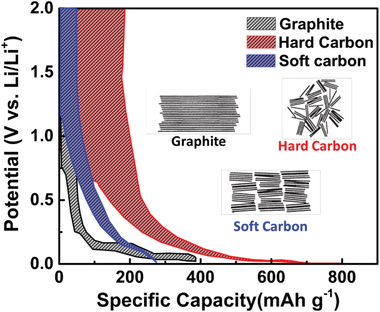
\includegraphics[width=\marginparwidth]{figures/application3/image2.png}
}
Multiple mechanisms are responsible for the storage of cation in the micro-porosity of the materials. Figure XX shows the different in the material potential vs Li during reduction of the electrodes. It is clear the absents of plateau which are associated with a phase change of a crystalline ordered structure, absent for the case of disordered carbon.
The most accredited storage mechanisms are adsorbtion, insertion and metal electrodeposition, as schematized in the Figure.
\begin{figure}
    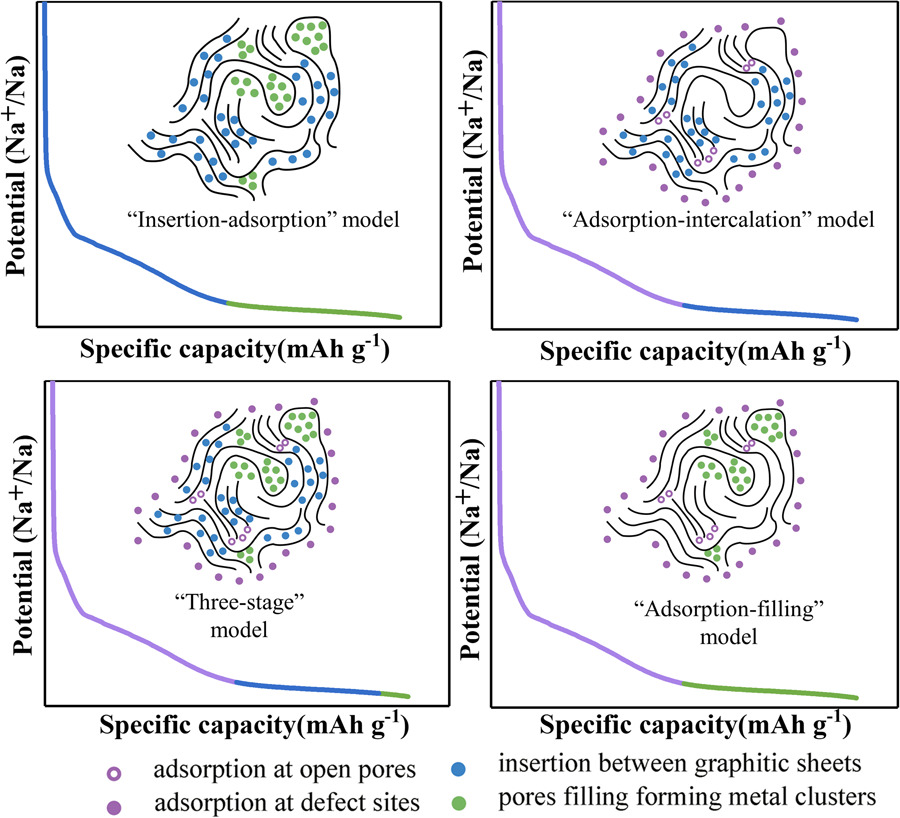
\includegraphics[width = \linewidth]{figures/application3/image3.png}
\end{figure}
It is still an open question which of this processes contribute the most and at which potential, and important information to design materials with higher capacity. Multiple theories are taken into account to far as reported in Figure.
\begin{figure}
    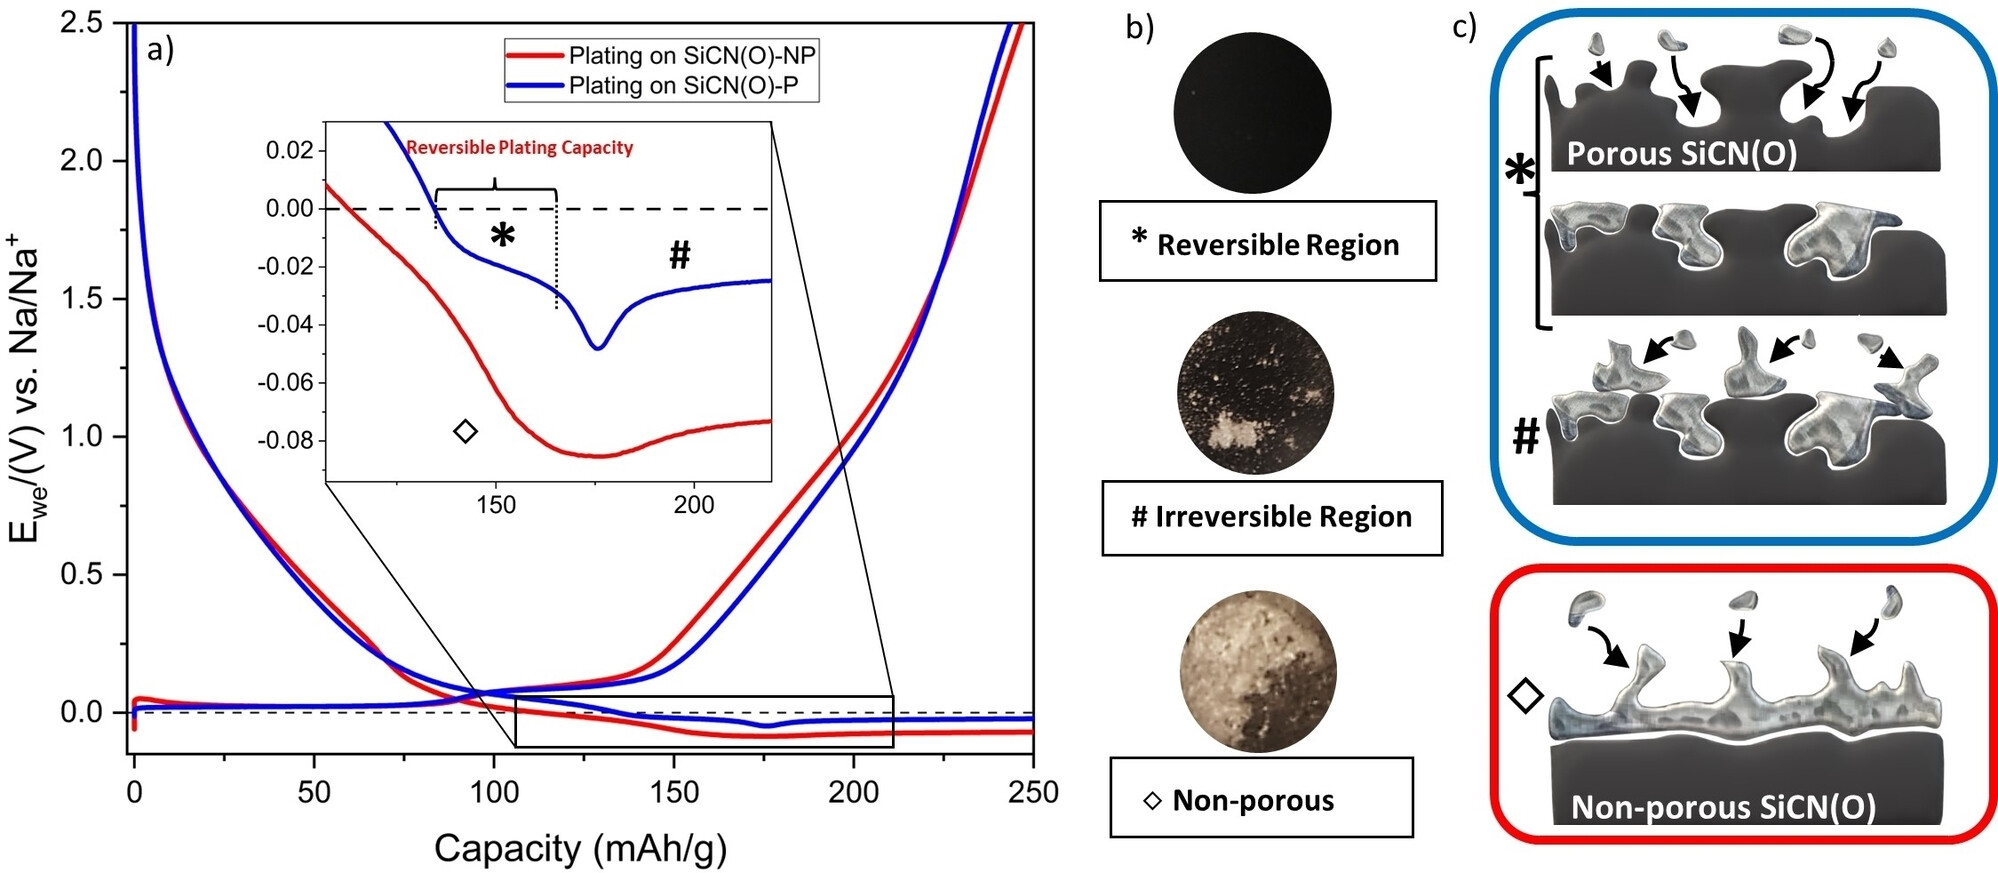
\includegraphics[width = \textwidth]{figures/application3/image4.png}
\end{figure}
Study such characteristics can only be done in operando condition with in situ tehcniques. Reserached used different mothodology for the identification of the position of the cation in the strucutre such as Nuclear Magnetic Resonance and Raman Spectroscopy. 

Silicon carbonitride, for the presence of Si-N bonding should a particularly good binding energy with atomic sodium, favorating the electrodeposition in the pore of the material. Marco Melzi et al demonstrated an increase of capacity when allowing the lower voltage limit to negative values, i.e. allowing electroceposition of Na to happen with high efficiency. Reducing the micro-porosity during the synthesis step removes the gain in performance. The goal of the project here describe was to find evidences of metal plating through the impedance during reduction and help infering the mechanism.

\subsection{Cell housing for three electrodes and optimization}
The measurement reported in Figure XX is a galvanostatic cyclation performed on a two-electrode half-cell with metalli sodium as counter electrode.

Descrivi la cella e le componenti.

While this cell is fine for the screening of material properties in therm of capacity and its retention, it is not suitable for electrochemistry investigation and more advance techniques like the Electrochemical Impedance Spectroscopy. This is espetially true for the case of sodium half-cells were the sodium metal -  electrolyte interface has an high impedance, up to two orders of magnitude than the silicon carbonitride electrode. For analyzing the impedance of the working electrode only a reference electrode has to be designed. For this work we started experimenting with a simple thin metallic sodium strip, positioned in the middle of the cell stack. To maintain the cell geomtery from the original pubblication a T-shaped three electrode was obtain from a Swagelock gas junction at the workshop of the University of Darmstadt. A section of the cell is reported in Figure XX. The results were at first interesting but we were not sure about the intruction of artifacts due to the size and thickness of the strip of sodium as reference electrode, comparable with the size of the electrodes itself. The pressure applied to the stack, in presence of glass fiber separator was high enough to easilly deform the sodium counter electrode. We later tried to use a microscopic reference electrode which should avoid the presence of artifacts according to the simulations. The details on it manifuacturing will be discessed in depth in the next section. This electrode is an insulated copper wire with only a section esposed (i.e. a disk of copper) on which sodium was in situ electrodeposited. Giving the concentration of the elecotrlyte of 1M constant as approximation during the cell evolution, it’s potential should be constant. The use of microscopic reference electrode for the relative measurement of electrode potential in batteries has gained a lot of interest in the last year. As explained in the introduction, alloying lithium with other metals, espetially the noble ones, produce a stable reference electrode. Unfortunalty sodium does not alloy with gold or alluminum, but only with tin. On the other hand sodium electrodeposits quite well on copper, in fact I got potential stability for months as will be reported later. The microscopic wire electrode was difficult to introduce in the T-shaped cell. For a simple assembling, the wire was screwed into a stainless-stell piston. Assembling such cells was difficult and gave inconsistent results and frequent short circuits. Finally I decided to move to a different geometry which I believe is much easier to assemble, leave more freedom on design and should grantee a better insulation: the pouch cell. The final designe is schematized in Figure XX.

Moving from a macroscopic to micriscopic refernce electrode was a choice based on the ideas that a microscopic reference might introduce artifacts in the impedance. As shown in the following section about the solid-electrolyte conductive interphase, an inductive loop was observed and the origini of such feature is often associated to geometrical considerations of the electrode positioning.

\begin{table}
\centering

\begin{tabular}{l l l l}
\toprule
\textbf{Nname} & \textbf{Type of cell} & \textbf{Electrodes} & \textbf{Type of reference electrode} \\
\toprule
Cell05 & IFAM Swagelok & SiCNO/Na & Strip of sodium metal \\
Cell10 & DTU Swagelok & SiCNO/Na & Strip of sodium metal \\
Cell13 & DTU Swagelok & SiCNO/Na & Strip of sodium metal \\
Cell35 & DTU Swagelok & SiCNO/Na & \thead[l]{Sodium electrodeposited on \\insulated copper wire (no piston) }\\
Cell36 & Pouch cell & SiCNO/Na & \thead[l]{Sodium electrodeposited on \\insulated copper wire (no piston) } \\
Cell38 & Pouch cell & SiCNO/Na & Strip of sodium metal \\
Cell39 & Pouch cell & SiCNO/Na & \thead[l]{Sodium electrodeposited on \\insulated copper wire (no piston) } \\
Cell40 & Pouch cell & Na/Na & \thead[l]{Sodium electrodeposited on \\insulated copper wire (no piston) } \\
\bottomrule

\end{tabular}

\end{table}


\subsection{Microscopic reference electrode of sodium}

 While the concept of microscopic reference electrodes is getting accepted for lithium redox copule   in non-aqueous solutions, the same it is not true for the case of sodium as described in chapter XXX. For this project we aimed to design a simple microscopic electrode using ready available materials in every laboratory or workshop. The reference material is metallic sodium electrodeposite in situ on the exposed face of an insulated copper wire. The wire here behaves only as current collector and mechanically strong substrate for the deposition of sodium. The entire length of the wire was insulated using two thermoplastic polymer strips, usually employed for the sealing of pouch cells. The copper wire, with a diameter of 130um, come from an inexpensive solder tip cleaner. 

\begin{figure}
    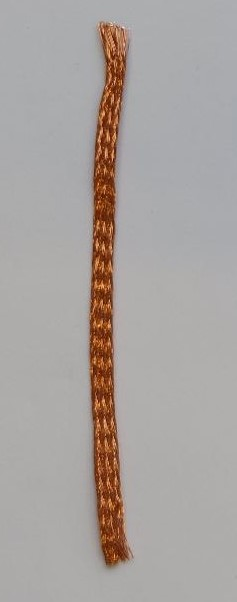
\includegraphics[width=2.1cm]{figures/application3/image5.1.jpg}
    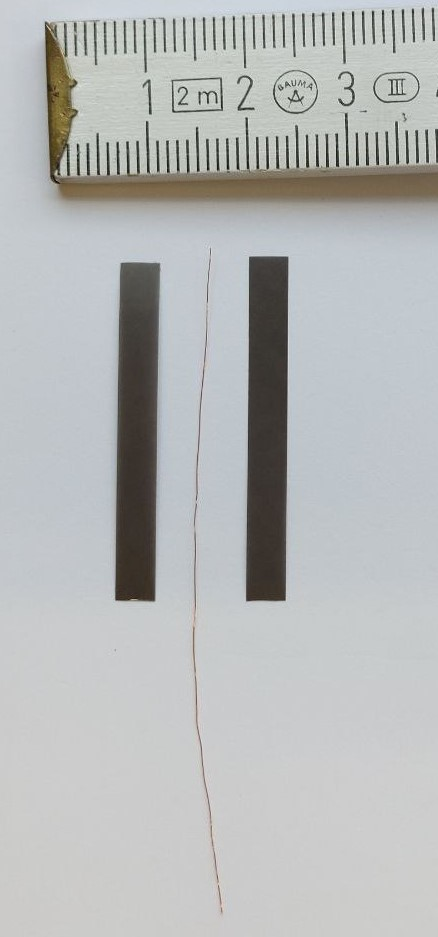
\includegraphics[width=2.5cm]{figures/application3/image5.2.jpg}
    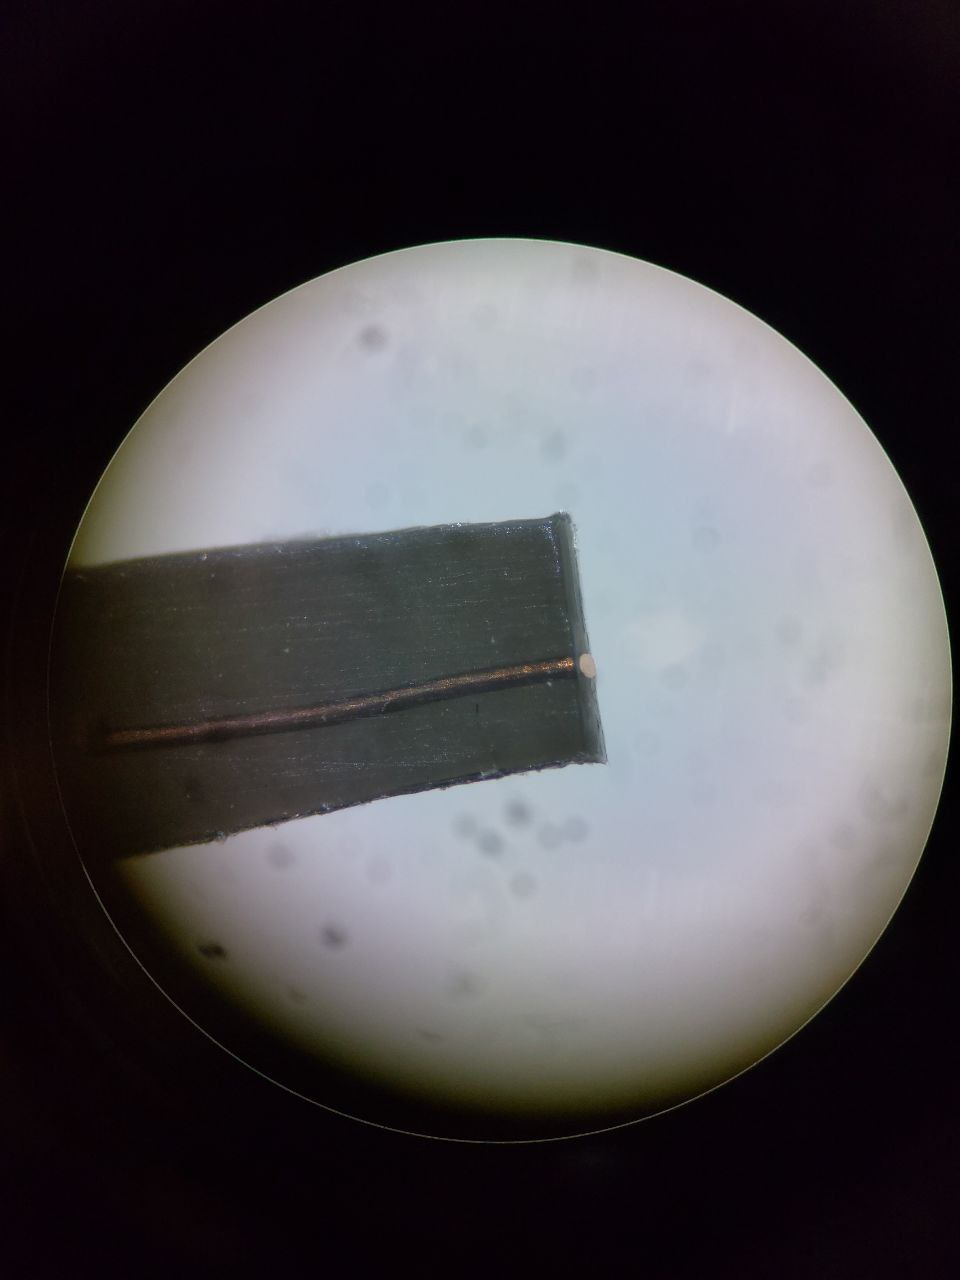
\includegraphics[width=4cm]{figures/application3/image5.3.jpg}
\end{figure}

The insulation of the wire was done putting the wire between to strips of polymeric strip longitudinal to the heating strip of an ultrasonic sealer for coffee bags. The Excess polymer were removed with a scalpel and a section of the wire exposed like shown in Figure XX. It takes a bit of practice to cut the section parallel to the axis and get aproximatly a circular section. Without checking on the optical microscope, one might end up with elliptical section resulted from non perpendicular cut and hence a much higher surface area.

For the electrodeposition the wire was connected to the working pole of a potentiostat using a disk of metallic lithium as counter (12 mm diameter) in a two-electrode configuration. The procedure was conducted with a two steps technique, first 10 minutes of potentiostatic set at -100mV and then 3 hours in galvanostatic with -50uA of current. It followed an open circuit technique. The reference electrode produced with such techniques were stable under parasitic  current of the potentiostat for 6 months.

\colorbox{BurntOrange}{Mettere le figure dell’OCV del reference}

\subsection{Time-varying impedance}

For this application I used the set-up Version 3 as discussed in the experimental section. The main drift consisted only of a galvanostatic reduction and oxidation with potential limitation without any rest or potentiostatic steps, to match the protocol used in a previous publication. The current was set to C/20 in respect to the theoretical capacity calculated as ????  in the potential windows of 0V to 2.5V vs Na. The multi-sine was generated with frequency components from 10mHz to 1kHz with 8 points per decades and remove frequencies that produce intermodulation. The amplitude was kept flat to arbitrary 1 V (see discussion for a comment on this choice) and crest factor optimized by random iteration of the phases. After loading the multi-sine on the waveform generator an amplitude of 80mV was set on the instrument. The multi-frequency signal was collected with a sampling frequency of 5kHz and the time-varying impedance estimated  through a Dynamic Multi-Frequency Analysis using a Symmetric Fermi-Dirac filter with 0.01Hz of bandwidth and n of 8.

\begin{figure}[h]
    \centering
    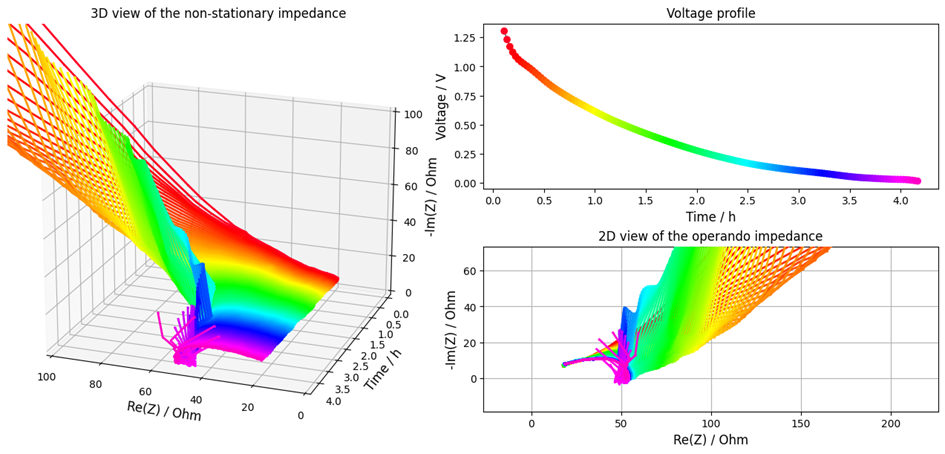
\includegraphics[width=\linewidth]{figures/application3/image6.png}
    \caption{Cell 10 first discharge after formation.}
    \label{fig:cell10_firs_cycle}
\end{figure}

\begin{figure}[h]
    \centering
    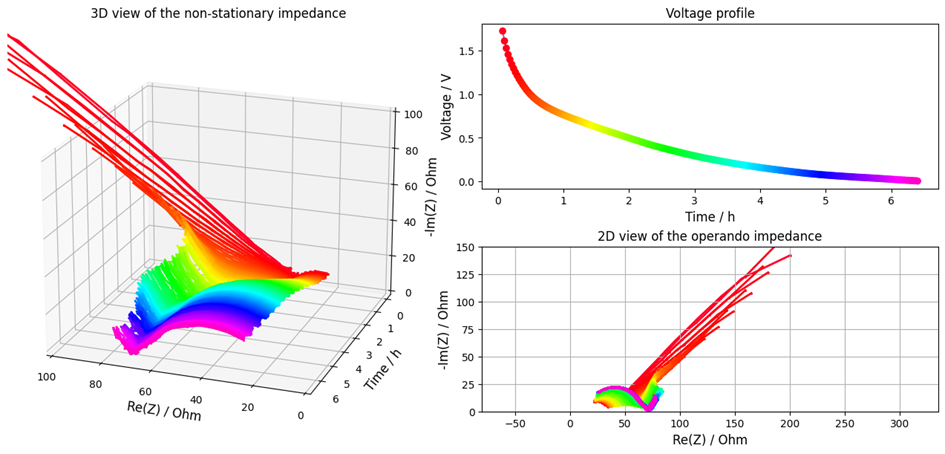
\includegraphics[width=\linewidth]{figures/application3/image7.png}
    \caption{Cell 35 first discharge after formation.}
    \label{fig:cell35_firs_cycle}
\end{figure}

\begin{figure}[h]
    \centering
    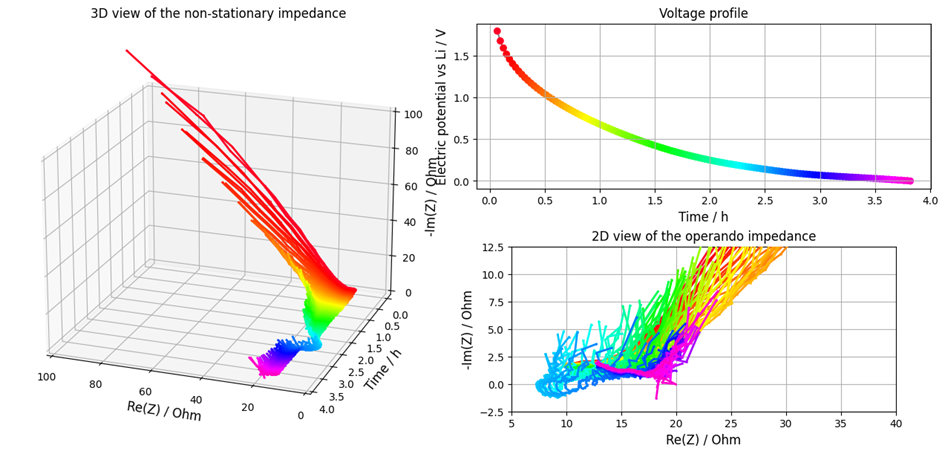
\includegraphics[width=\linewidth]{figures/application3/image8.png}
    \caption{Cell 36 first discharge after formation.}
    \label{fig:cell36_firs_cycle}
\end{figure}

\begin{figure}[h]
    \centering
    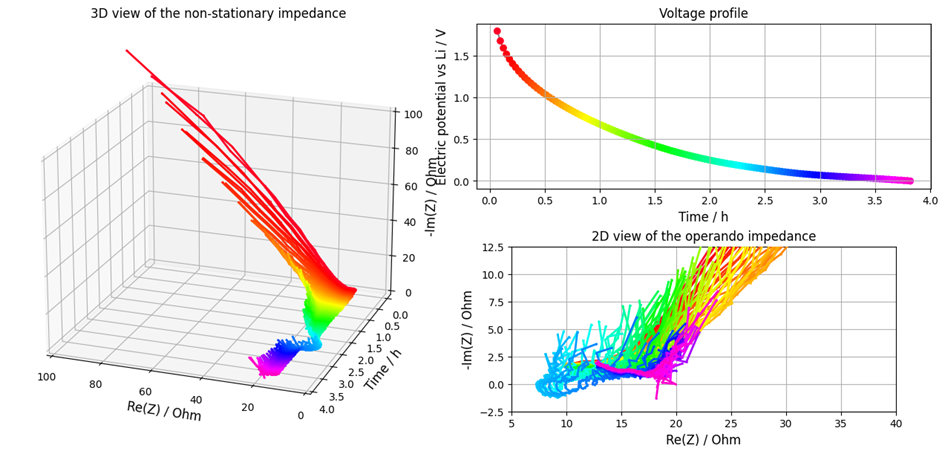
\includegraphics[width=\linewidth]{figures/application3/image8.png}
    \caption{Cell 38 first discharge after formation.}
    \label{fig:cell38_firs_cycle}
\end{figure}

\begin{figure}[h]
    \centering
    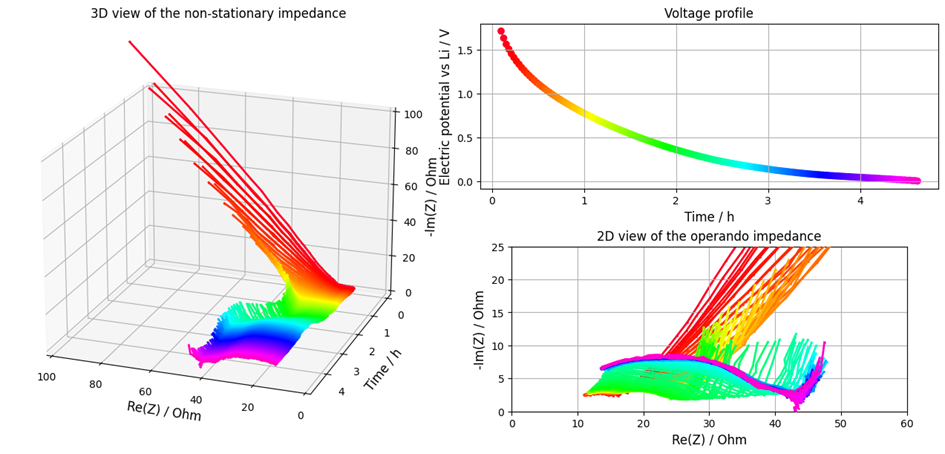
\includegraphics[width=\linewidth]{figures/application3/image9.png}
    \caption{Cell 39 first discharge after formation.}
    \label{fig:cell39_firs_cycle}
\end{figure}

\subsection{Sodium electrodeposition on sodium substrate}

\begin{figure}[h]
    \centering
    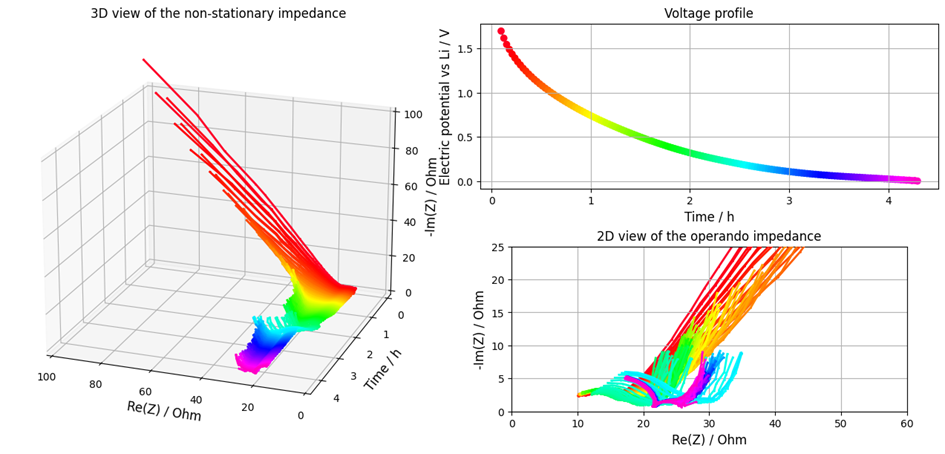
\includegraphics[width=\linewidth]{figures/application3/image10.png}

\end{figure}

\begin{figure}[h]
    \centering
    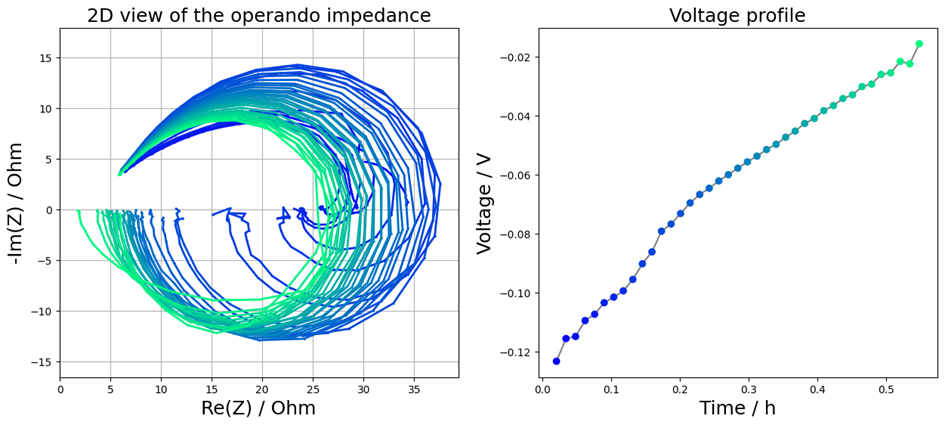
\includegraphics[width=\linewidth]{figures/application3/image11.png}
\end{figure}

\begin{figure}[h]
    \centering
    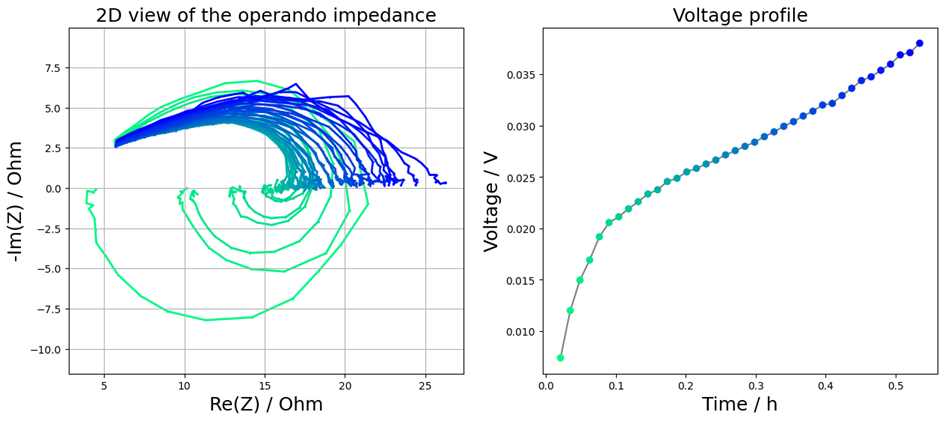
\includegraphics[width=\linewidth]{figures/application3/image12.png}
\end{figure}

\begin{figure}[h]
    \centering
    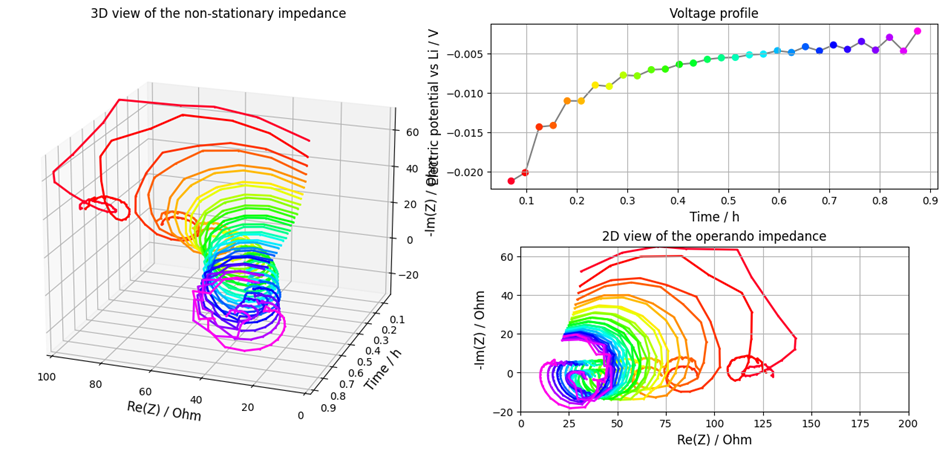
\includegraphics[width=\linewidth]{figures/application3/image13.png}
\end{figure}

\begin{figure}[h]
    \centering
    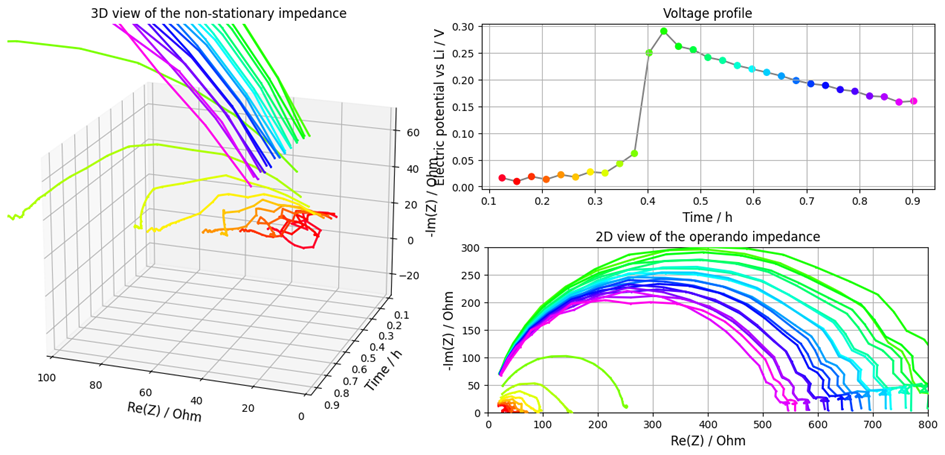
\includegraphics[width=\linewidth]{figures/application3/image14.png}
\end{figure}

\subsection{Time-Varying impedance during SEI formation}

\begin{figure}[h]
    \centering
    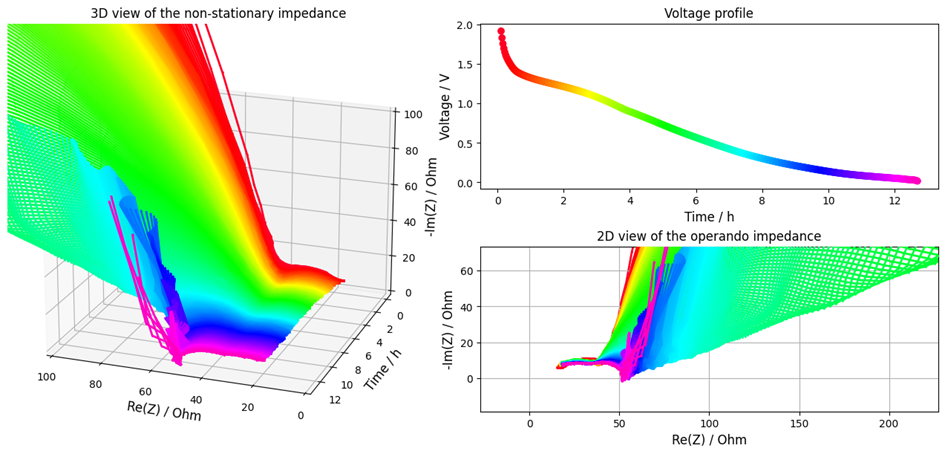
\includegraphics[width=\linewidth]{figures/application3/image15.png}
    \caption{Cell 10 formation.}
    \label{fig:cell10_formation}
\end{figure}

\begin{figure}[h]
    \centering
    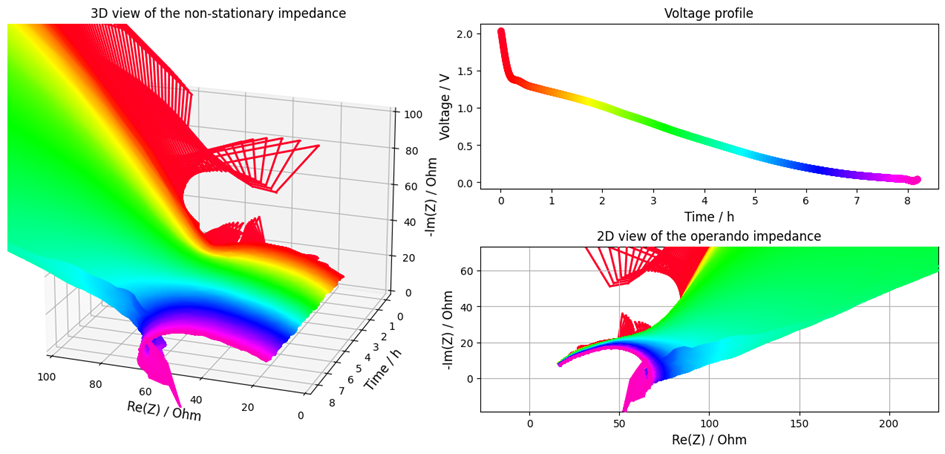
\includegraphics[width=\linewidth]{figures/application3/image16.png}
    \caption{Cell 13 formation.}
    \label{fig:cell13_formation}
\end{figure}

\begin{figure}[h]
    \centering
    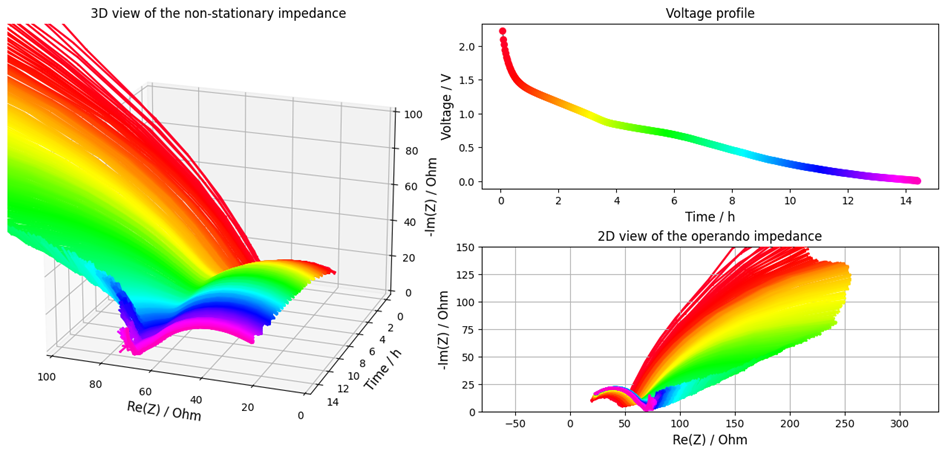
\includegraphics[width=\linewidth]{figures/application3/image17.png}
    \caption{Cell 35 formation.}
    \label{fig:cell35_formation}
\end{figure}

\begin{figure}[h]
    \centering
    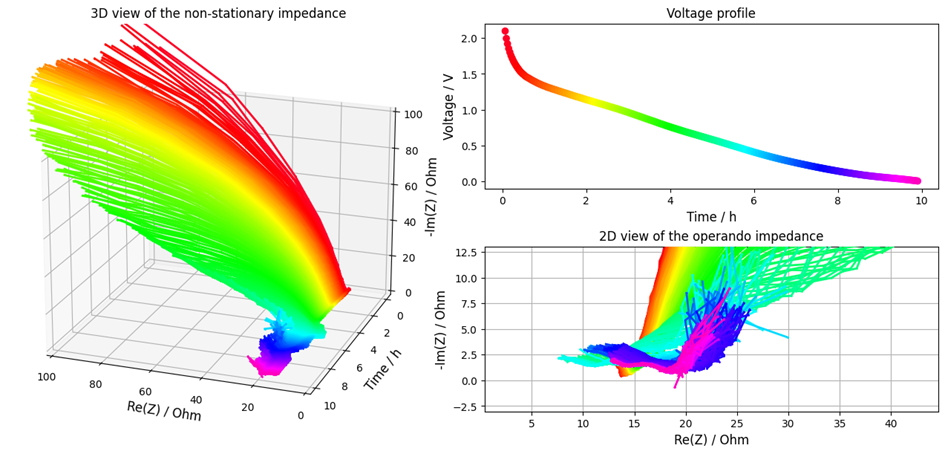
\includegraphics[width=\linewidth]{figures/application3/image18.png}
    \caption{Cell 36 formation.}
    \label{fig:cell36_formation}
\end{figure}

\begin{figure}[h]
    \centering
    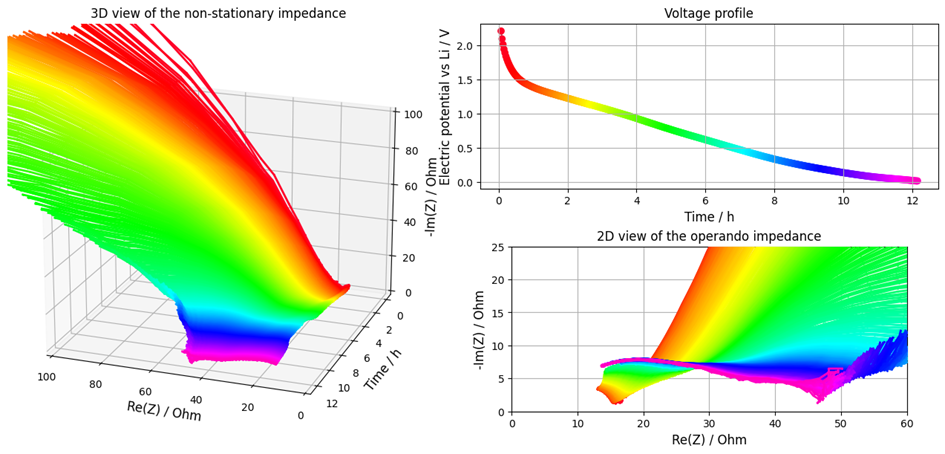
\includegraphics[width=\linewidth]{figures/application3/image19.png}
    \caption{Cell 38 formation.}
    \label{fig:cell38_formation}
\end{figure}

\begin{figure}[h]
    \centering
    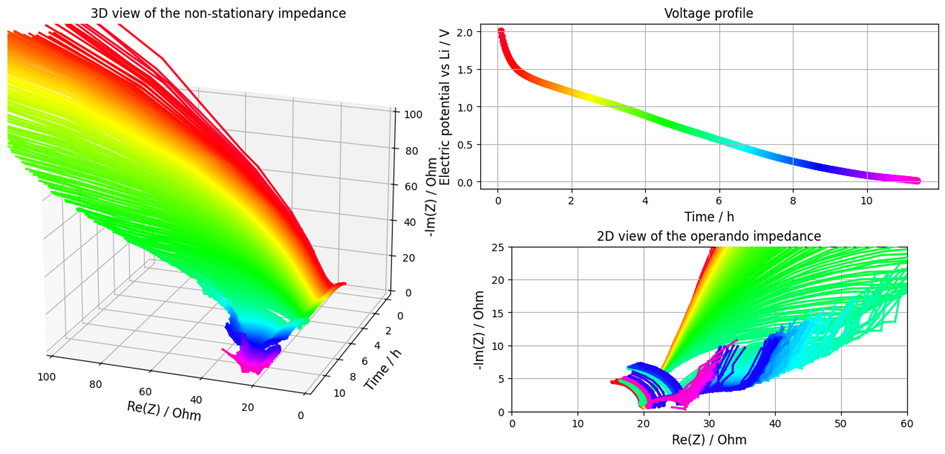
\includegraphics[width=\linewidth]{figures/application3/image20.png}
    \caption{Cell 39 formation.}
    \label{fig:cell39_formation}
\end{figure}